% =============================================================================
% =  Related Works
% =============================================================================

\section{Related Work} \label{sectionRelatedWork}

In our research, we are running with the assumption that Maintainability Index (MI) is our primary indicator. Consequently, we will look for the correlation between the MI and other Pylint scores.

\subsection{Considering Data Sets}

When exploring the correlations between maintainability and refactoring, many sources are available for research. For example, some researchers have looked at proprietary systems as they evolve, while others have chosen open-source code available to the general public.

A study conducted by Baishakhi Ray, Daryl Posnett, Premkumar Devanbu, and Vladimir Filkov begins by programmatically collecting a sample set of projects on GitHub that vary in languages. Then the group of projects is appropriately thinned out, resulting in a final set used for the review. The results are then studied for the impact different programming languages may have on the code quality \cite{baishakhi:2017}. Finally, their research determined which languages were more prone to defects and which individual languages were more related to individual bugs rather than bugs overall.

The authors of ``Predicting Maintainability with Object-Oriented Metrics - An Empirical Comparison'' performed a similar study to what we are doing here. Their study focuses on object-oriented software (specifically C/C++ and Java) and correlation analysis between object-oriented metrics and software maintainability. Janke et al. looked for the best metrics to predict maintainability \cite{janke:2003}. That study focused on a few hand-picked software systems with an analysis of the changelogs. Our study, in contrast, will be of a larger scale (about 50 software systems) and focused solely on Python-heavy projects.

\subsection{Design Patterns \& Software Quality}

In the paper ``Impact of design patterns on software quality: a systematic literature review'' the authors compared the use of design patterns to software evolution and maintainability. They found that design patterns provided flexibility when reviewing changes that extended (evolved) software \cite{wedyan:2020}.

\vspace{0.25cm}
\begin{displayquote}
  ``Changes performed in a class can be corrective, adaptive, perfective, or preventive. These changes can occur due to new requirements, debugging, changes that propagate from changes in other classes and refactoring.''
\end{displayquote}
\vspace{0.25cm}

Wedyan and Abufakher found that there were two reasons that a class had more frequent changes \cite{wedyan:2020}:

\vspace{0.25cm}
\begin{enumerate}
    \item The class was easy to extend.
    \item The class correlated to other classes (raising alarms about class modularity).
\end{enumerate}
\vspace{0.25cm}

With these findings in mind, we intentionally aim to focus our research on changes for system extensions and adaptations rather than bug fixes that appeared to be more considerable change due to high coupling. This paper centers on Refactor scores (code smells) rather than Error scores (bugs) within the system.

\subsection{Software Architecture \& Maintainability}

In the research done in ``Software Architecture Metrics: A Literature Review'', the authors discuss how early detection of issues within the software's architecture is key to mitigating the risk of poor performance and can lower the cost of repairing faults \cite{coulin:2019}. While most developers have had access to these metrics for several decades, the industry and open-source community have not commonly adopted their use for keeping code in easy-to-work-with conditions.

The review done by Coulin et al. called out five essential qualities of software architecture \cite{coulin:2019}:

\vspace{0.25cm}
\begin{enumerate}
    \item Maintainability
    \item Extensibility
    \item Simplicity, Understandability
    \item Re-usability
    \item Performance
\end{enumerate}
\vspace{0.25cm}

Focusing on these qualities can narrow down the choice between different design options to an ideal solution. Keeping these five qualities in top-of-mind for new (and changed) code allows for easier future development and evolution of the software system.

ISO/IEC 25010:2011 is a detailed standard for software quality that contains eight product quality characteristics  \cite{iso/iec:25010:2011}. Each characteristic is further comprised of various sub-characteristics. ``Fig.~\ref{figProductQualityModel}'' lists these characteristics, with maintainability being one of the most significant characteristics in some studies \cite{gupta:2021}, \cite{adewumi:2016}.

\begin{figure}[ht]
  \centerline{
    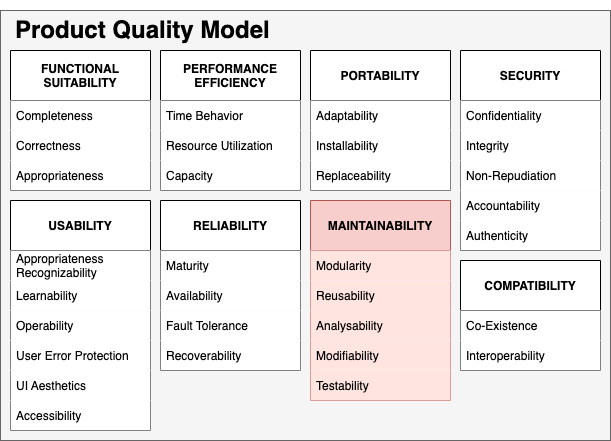
\includegraphics[width=0.7\columnwidth]{ProductQualityModel.png}
  }
  \caption{The eight product quality characteristics and sub-characteristics.}
  \label{figProductQualityModel}
\end{figure}
